\documentclass[11pt,letterpaper]{article}
\usepackage[english]{babel}
\usepackage[utf8]{inputenc}
\usepackage{fancyhdr}
\usepackage[margin=1in]{geometry}
\usepackage{enumitem}
\usepackage{amsmath}
\usepackage{graphicx}
\usepackage{setspace} 
\usepackage{pdfpages}
\usepackage{xcolor}
\onehalfspacing
 
\pagestyle{fancy}
\fancyhf{}
\lhead{CS\&SS 569 HW 2}
\rhead{Nan Tang (1662478)}
\rfoot{Page \thepage}
 

\title{CS\&SS 569 Homework 2}
\author{Nan Tang 1662478}
\date{\today}
 
 
\begin{document}
\maketitle
 
\subsection*{Abstract}
The Dataset I used for this homework named House Sales in King County. It contains all the deal price for houses in King count between May 2014 and May 2015. The dataset is suitable for evaluating a multivariate linear regression. In this short research, I am going to figure out significant predictors for house price and compare the predicative power of them. Visualize multivariate relationship is difficult, therefore, I reduce the oveall dimension of predictors but try to include as many dimensions as I can in multiples or single graphs. Codes are included at last few pages. 

\subsection*{Heatmap of Coefficients Matrix (ggplot2)}
\includegraphics[scale=0.8]{HW2-1.pdf}

\noindent For any linear regression, using twenty predictors has high risk of multi-colinearity. Therefore, filtering out insignificant or variables with high inflation factor is necessary. I choose $geom_tile$ as a heat map to display the correlation coefficients matrix. I choose the sequential color scale from color brewer to represent values of correlation coefficients. The more positive value is darker in blue, while the more negative value is brighter in yellow. Yellow and blue are two distinctive values, therefore they can be chosen as two poles, while the midpoint green represents non-correlation. Different from traditional visuals of correlation matrix where use darkest color on diagonal (since correlation equals 1 is the highest value), I use light gray for diagonal, simply because these values are meaningless. \\

\noindent It is easy to perceive from this visual that square feet of living room has strongest linear relationship with house price. Meanwhile it is strongly co-linear with other variables such as number of bedrooms, bathroom, square feet of house above ground and grade. Therefore I will drop all those co-related variables and leave square feet of living room as predictor. 


\subsection*{Visualize Robust Linear Regression (ggplot2)}
\includegraphics[scale=0.8]{HW2-2.pdf}

\noindent This is basically a draft plot (please do not grade on it). Upper half of the grid represents price - square feet of living room relationship with multiple levels of floors for inland houses, the lower half is for waterfront house. As we can perceive from the the plot, some level of floors has not enough sample for the model, therefore I planed to converge  levels of floors into two levels. 

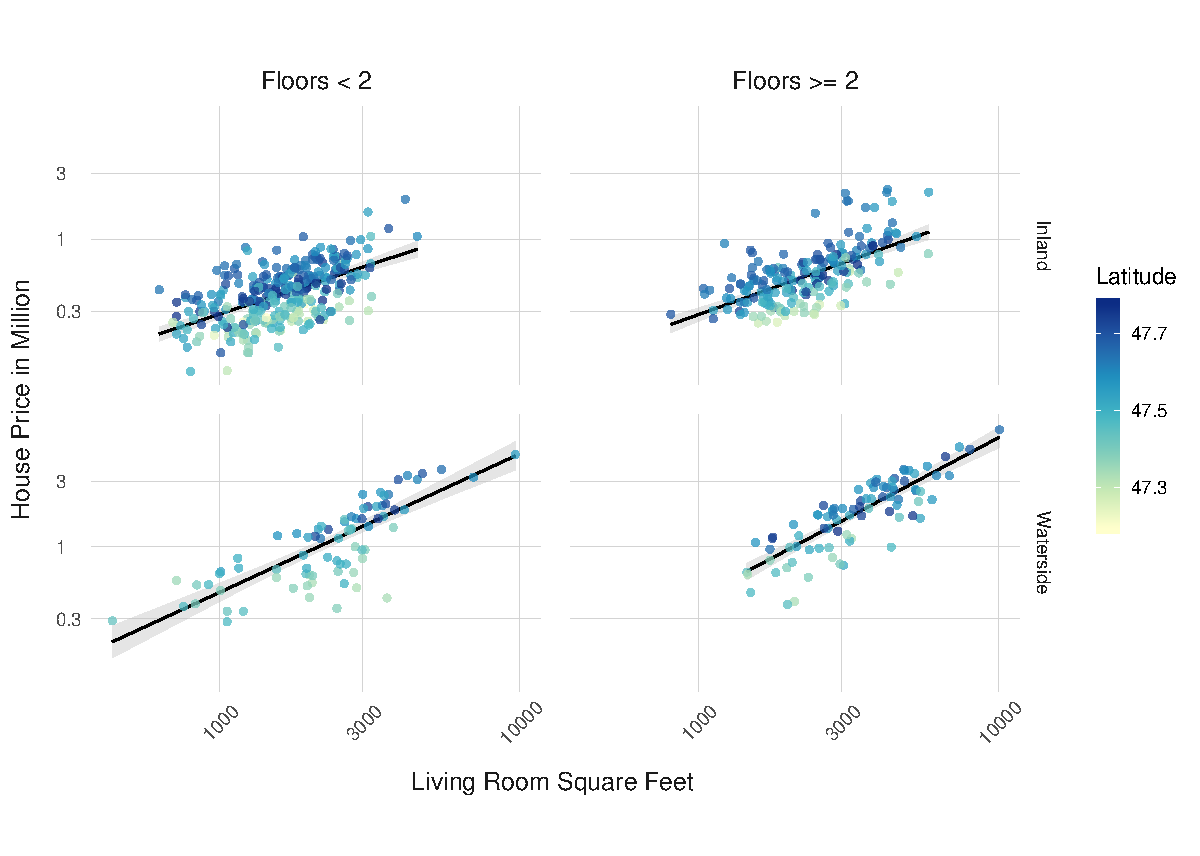
\includegraphics[scale=0.8]{hw2-3.pdf}

\noindent Color represents latitude of the house. Sequential color scale from yellow to blue covers latitude of range $N 47.2 - N 47.7$. I chose this color scale for its intuitive sense that blue is colder and yellow is warmer, matching with higher latitude and lower latitude. \\

\noindent The robust regression plot shows significant effect of location (include latitude and whether in front of water) on house price. Though transparency has some degree of effect on identify the true color of that spot, distinctive clusters of yellow, indigo and blue points are shown. The slope and intercept of regression line for waterfront is clearly higher than inland house. 

\subsection*{Comparison between Levels of  Categorical Variables (tile)}

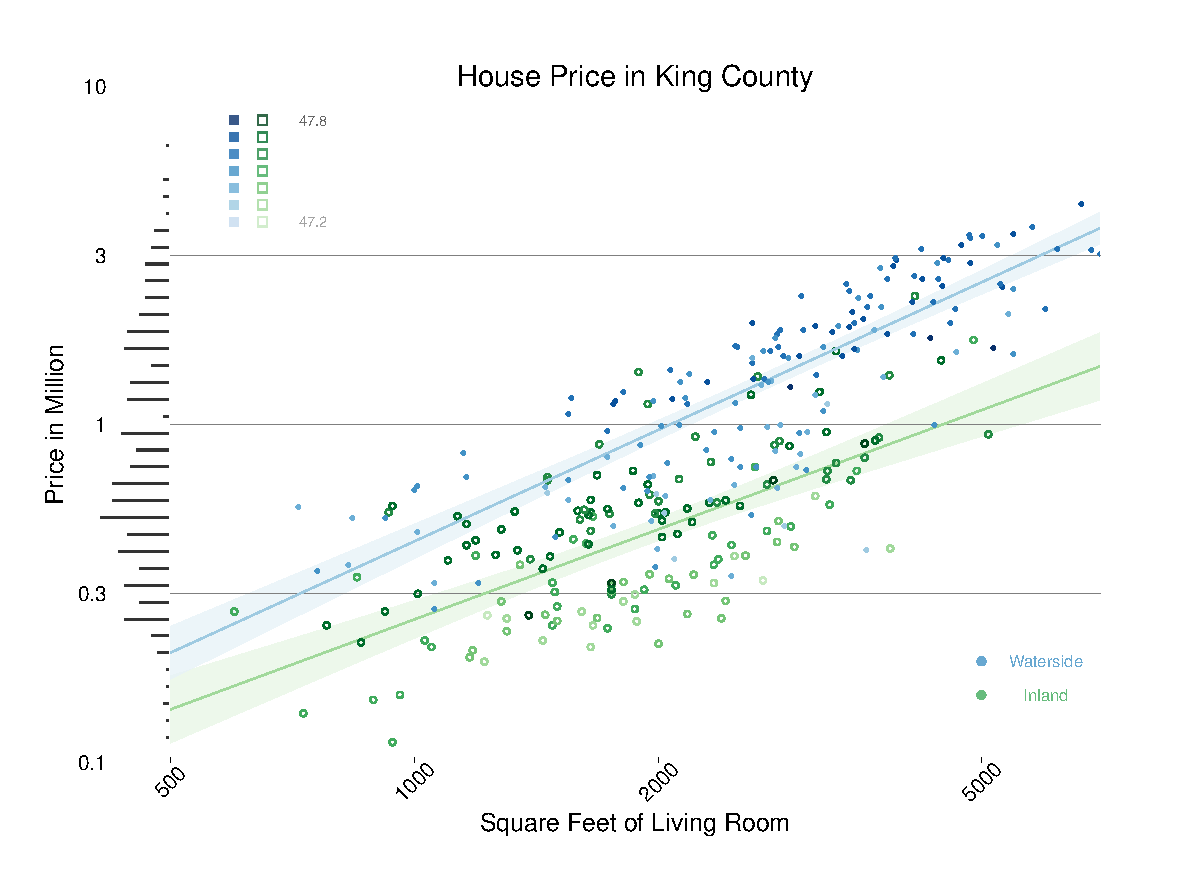
\includegraphics[scale=0.8]{HW2-4.pdf}

\noindent Basically, I combined four dimensions of data into one scatter plot. I chose green and blue to represent inland and waterside house for intuitiveness. Color saturation are used to represent latitude in this case. Higher saturation implies higher latitude. One of the issue is when both green and blue has low saturation (too much white), it is difficult to distinguish in between. Therefore I chose two shapes of spot to represent whether its inland or waterside. Though shape is not a good character to display categorical variables, I believe in this case, where two clusters are somehow far away from each other, hollow dots can stand out of solid ones. I also used vertical legend for latitude for intuitive sense. 

\newpage

\subsection*{Code in R}
\begin{verbatim}
## visualize paired correlation matrix

## Prepare dataset and correlation matrix
house_new <-house_dt %>% 
  dplyr::select(price, bedrooms, bathrooms,sqft_living, sqft_lot, 
                sqft_above, sqft_basement,floors, waterfront, 
                condition, grade, yr_built, yr_renovated, lat, long)

house_corr <- cor(house_new)
house_corr_df <- melt(house_corr)
house_corr_df <- house_corr_df %>% 
  mutate(value = replace(value, value==1, NA))

p1 <- ggplot(data=house_corr_df, mapping=aes(x=Var1, y=Var2, fill=value)) +
  geom_tile(color='white', size=0.75) + 
  scale_fill_distiller(palette = "YlGnBu", breaks=seq(-0.3, 0.9, 0.3), 
                       name=NULL, na.value='gray95', direction = 1) +
  ggtitle('Matrix of Correlation Coefficients') +
  theme (
    axis.text.x = element_text(angle=45, vjust=0.6),
    axis.text.y = element_text(angle=0, hjust=0.6), 
    axis.ticks = element_blank(),
    axis.title = element_blank(),
    plot.title = element_text( hjust=0.5, vjust=0),
    legend.text = element_text(face='bold'),
    legend.key.width = grid::unit(0.3,'cm'),
    panel.background = element_blank(),
    panel.border=element_blank(),
    panel.grid.major = element_blank()
  )
  
  
## Visualize robust regression between price and couple of factors
## Use grid of multiples to show categorical variables

## Prepare dataset and sample 500 obs from original data 
house_reg_dt <- house_new %>% 
  dplyr::select(price, sqft_living, waterfront, lat, floors) %>%
  mutate(waterfront = as.factor(ifelse(waterfront == '0', 'Inland', 'Waterside'))) %>%
  mutate(floors = ifelse(floors < 2, 'Floors < 2', 'Floors >= 2')) %>%
  mutate(floors = as.factor(floors))

sp_index <- which(house_reg_dt$waterfront=='Waterside')
sp_index <- c(sp_index, sample(which(house_reg_dt$waterfront=='Inland'), 500))
house_reg_sp <- house_reg_dt[sp_index,]

title_col <- 'gray10'
grid_col <- 'lightgray'

p3 <- ggplot(data=house_reg_sp, aes(x=sqft_living, y=price)) +
  geom_smooth(method=MASS::rlm, method.args=list(method="MM"),
              formula = y~x, size=0.5, color='black', level=0.95, fill='gray75') +
  geom_point(aes(col=lat), alpha=0.75, shape=16) + 
  scale_x_log10(name='Logarithm of Living Room Square Feet ') +
  scale_y_log10(breaks=c(3e+05, 1e+06, 3E+06), 
                labels=c(0.3, 1, 3),name='Logarithm of Price in Million') +
  scale_color_distiller(palette = 'YlGnBu', direction = 1, name='Latitude',
                        breaks=c(47.3, 47.5, 47.7))  +
  facet_grid(cols=vars(floors), rows=vars(waterfront)) +
  theme(
    aspect.ratio = ((1 + sqrt(5))/2)^(-1),
    axis.ticks = element_blank(),
    axis.text.x = element_text(angle=45, vjust=0.6),
    axis.title.x = element_text(margin=margin(t=7), size=12, color=title_col),
    axis.ticks.y = element_blank(),
    axis.text.y = element_text(hjust=0),
    axis.title.y = element_text(margin=margin(r=7), size=12, color=title_col),
    
    legend.key.width = grid::unit(0.4,'cm'),
    legend.key.height =  grid::unit(0.8,'cm'),
    
    strip.background = element_blank(),
    strip.text.x = element_text(size=12, color=title_col), 
    strip.placement = "outside",      
    
    panel.spacing.x = unit(1, "lines"), 
    panel.spacing.y = unit(1, "lines"),
    panel.background = element_rect(fill = "white"),
    panel.grid.major.x = element_line(color=grid_col, size=0.1),
    panel.grid.major.y = element_line(color=grid_col, size=0.1),
  )


## Use tile and one plot to compare categorical variables 
## Prepare dataset and sample 300 obs from origin data
sp_index <- which(house_reg_dt$waterfront=='Waterside')
sp_index <- c(sp_index, sample(which(house_reg_dt$waterfront=='Inland'), 150))
house_reg_sp <- house_reg_dt[sp_index,]

inland_sp <- house_reg_sp %>% 
  filter(waterfront == 'Inland')
waterside_sp <- house_reg_sp %>%
  filter(waterfront == 'Waterside')

inland_lat_col <- brewer.pal(9, 'Greens')[3:9]
inland_col_sys <- mapvalues(inland_sp$lat_intv, from=levels(inland_sp$lat_intv), to=inland_lat_col)
inland_col_sys <- as.character(inland_col_sys)

water_lat_col <- brewer.pal(9, 'Blues')[3:9]
water_col_sys <- mapvalues(waterside_sp$lat_intv, from=levels(waterside_sp$lat_intv), to=water_lat_col)
water_col_sys <- as.character(water_col_sys)

trace1 <- scatter(
  x = inland_sp$sqft_living,
  y = log10(inland_sp$price),
  fit = list(method="mmest", ci = 0.95, col=inland_lat_col[2]),
  col = inland_col_sys,
  pch = rep(1, ncol=length(inland_sp)),
  plot = 1
)

trace2 <- scatter(
  x = waterside_sp$sqft_living,
  y = log10(waterside_sp$price),
  fit = list(method="mmest", ci = 0.95, col=water_lat_col[2]),
  col = water_col_sys,
  pch = rep(16, ncol=length(waterside_sp)),
  plot = 1
)

legendSymbols1 <- pointsTile(
  y = c(5.3, 5.2),
  x = c(5000, 5000),
  col = c(water_lat_col[4], inland_lat_col[4]),
  cex = 1.5, 
  pch = 16,
  plot = 1
)

legendLabels1 <- textTile(
  labels = c('Waterside', 'Inland'),
  x = c(6000, 6000),
  y = c(5.3, 5.2),
  col = c(water_lat_col[4], inland_lat_col[4]),
  fontsize = 8,
  plot=1
)

legendSymbols2 <- pointsTile(
  y = c(seq(6.9, 6.6, -0.05), seq(6.9, 6.6, -0.05)),
  x = c(rep(600, times=7), rep(650, times=7)),
  col = c(rev(water_lat_col),rev(inland_lat_col)),
  cex = 1.5, 
  pch = c(rep(15, times=7), rep(0, times=7)),
  plot = 1
)

legendlabels2 <- textTile(
  labels = c('47.8', '47.2'),
  y = c(6.9, 6.6),
  x = c(750, 750),
  col = c('gray25', 'gray 55'),
  fontsize = 7,
  plot = 1
)

rug_y <- rugTile(
  y = log10(house_reg_sp$price),
  type='dots',
  thickness=2,
  plot = 1
)

tile(
  trace1,
  trace2,
  legendSymbols1,
  legendLabels1,
  legendSymbols2,
  legendlabels2,
  rug_y,
  
  xaxis = list(log = TRUE, fontsize = 10, rot = 45,
               tick.length= 0.2, major=FALSE),
  xaxistitle = list(labels = c('Square Feet of Living Room'), fontsize = 10),
  yaxis = list(fontsize = 10, labels=c(0.1, 0.3, 1, 3, 10), major=FALSE),
  yaxistitle = list(labels = c('Price in Million'), fontsize = 10),
  rightaxis = list(labels=c('ee')),
  plottitle = list(labels = c('House Price in King County'), fontsize = 10),
  gridlines = list(type='y'),

  limits = c(500, 7000, 5, 7),
  RxC = c(1 ,1),
  height = list(plot=1.6, plottitle=1, xaxistitle=1),
  width = list(plot=2.2, yaxistitle=0.5, rightborder=4),
  
  output=list(file='HW2-4', width=8)
)
\end{verbatim}
 
 
 
 
 
\end{document}